\chapter{Integrating the GLV model at criticality}
\label{chap:rescaling}

The Generalized Lotka--Volterra (GLV) system that governs the dynamics of the
interacting nodes of our network reads
\begin{equation}
    \dot{x}_i = x_i \left( 1 - x_i + \sum_j W_{ij} x_j \right),
    \label{eq:glv}
\end{equation}
Here $x_i \ge 0$ is the abundance of node $i$. The term $1 - x_i$ is its own logistic
growth, an intrinsic rate of one with a self-limitation $-x_i$ that would cap an
isolated node at $x_i = 1$, and $\sum_j W_{ij} x_j$ is its coupling to the rest of the
network, cooperative where $W_{ij} > 0$ and competitive where $W_{ij} < 0$. The
interaction matrix is built as a product of two pieces, $W_{ij} = A_{ij}\,\alpha_{ij}$.
The adjacency matrix $A$ fixes the topology: $A_{ij} = 1$ when nodes $i$ and $j$ are
connected and $0$ otherwise, drawn from a configuration model with a prescribed degree
distribution and mean degree $C$. The weight on each existing edge is
$\alpha_{ij} = \mu/C + (\sigma/\sqrt{C})\,z_{ij}$, with $z_{ij}$ independent standard
Gaussians, so $\mu$ sets the mean (cooperative) strength of an interaction and $\sigma$
its disorder, while the diagonal $W_{ii}$ is zero. The factors $1/C$ and $1/\sqrt{C}$
keep the interaction field $\sum_j W_{ij} x_j$ of order one as the mean degree $C$
grows: a node has about $C$ neighbours, so the $C$ contributions of mean $\mu/C$ sum to
a mean of order $\mu$, and their variances $\sigma^2/C$ to order $\sigma^2$. The two
directions of an edge are drawn independently, so the couplings have zero reciprocity,
$\gamma = 0$. Our goal is to probe the system at and
beyond the cooperative critical point $\mu_c$, where the macroscopic abundance
stops equilibrating. This is the regime in which a direct numerical integration
of \eqref{eq:glv} fails: as $\mu \to \mu_c^{-}$ the total abundance grows without
bound, and for $\mu > \mu_c$ it diverges in finite time, so any explicit solver
is driven either to vanishing step sizes or to floating-point overflow.

The strategy of this chapter is to reorganize the dynamics so that the
divergence no longer obstructs the integration, rather than to attack it directly.
We split the system into a bounded ``shape'' degree of freedom living on the
probability simplex and an unbounded ``scale'' degree of freedom carrying the
total abundance, and we then stretch time so that the shape is governed by a
closed, bounded set of equations. This does not make the scale finite: the
total abundance still diverges for $\mu > \mu_c$. But it changes the character
of the divergence. The finite-time singularity that breaks explicit solvers in
physical time becomes a smooth, asymptotic growth in the new time variable. The
bounded shape can then be integrated stably through $\mu_c$, and the physical
trajectories $x(t)$ reconstructed from it wherever the scale remains numerically
representable.

\section{Mapping to the probability simplex and time rescaling}
\label{sec:simplex-mapping}

We separate scale from shape by introducing the total abundance $M(t)$ and the
relative fractions $y_i(t)$,
\begin{equation}
    M(t) = \sum_j x_j(t), \qquad
    y_i(t) = \frac{x_i(t)}{M(t)} .
    \label{eq:rescaling-def}
\end{equation}
By construction the fractions are confined to the probability simplex,
\begin{equation}
    y_i(t) \ge 0 \quad \forall t, \qquad \sum_j y_j(t) = 1,
\end{equation}
so they remain bounded for all $\mu$, including the divergent regime. The
projection of a GLV flow onto the simplex is, up to the choice of time
parametrization, a replicator equation, in the sense of Hofbauer's classical
correspondence between Lotka--Volterra and replicator dynamics
\cite{hofbauer81}. What is unusual here is that we keep the equation for the
total abundance, which is normally discarded because away from criticality it is
finite, and so irrelevant.

Carrying \eqref{eq:rescaling-def} through \eqref{eq:glv} (the step-by-step
algebra is given in Appendix~\ref{app:derivation}) leaves the shape dynamics
still coupled to the macroscopic envelope $M(t)$ through a multiplicative
factor. Since $M(t)$ is the quantity that diverges, this is not yet
enough. We therefore stretch time as well, by defining a new variable
$\tau$ through
\begin{equation}
    \frac{d\tau}{dt} = M(t).
    \label{eq:time-rescaling}
\end{equation}
Because $M$ grows without bound, a bounded range of physical time corresponds to an
unbounded range of $\tau$: the finite interval up to the blow-up time $t^\ast$ maps
onto the whole rescaled axis $\tau \in [0,\infty)$. Integrating $dt/d\tau = 1/M$
confirms this, since $t(\tau) \to t^\ast$ from below as $\tau \to \infty$. The
singularity at $t^\ast$ is therefore moved to $\tau = \infty$ and approached
smoothly, which lets an adaptive solver pass through the critical regime without its
step size collapsing. With this change of variables the system
\eqref{eq:glv} becomes
\begin{align}
    \frac{dy_i}{d\tau} &= y_i \left[ \sum_{j=1}^N W_{ij} y_j - y^{\!\top} W y - y_i + y^{\!\top} y \right],
    \label{eq:dydtau} \\[4pt]
    \frac{dM}{d\tau}   &= 1 + M \left( y^{\!\top} W y - y^{\!\top} y \right),
    \label{eq:dMdtau} \\[4pt]
    \frac{dt}{d\tau}   &= \frac{1}{M}.
    \label{eq:dtdtau}
\end{align}
The shape dynamics \eqref{eq:dydtau} can be written compactly using
element-wise multiplication ($\odot$) and the all-ones vector $\mathbf{1}$,
\begin{equation}
    \frac{dy}{d\tau} = y \odot \left[ Wy - (y^{\!\top} W y)\,\mathbf{1} - y + (y^{\!\top} y)\,\mathbf{1} \right].
    \label{eq:dydtau-vec}
\end{equation}

The crucial structural feature is that \eqref{eq:dydtau}--\eqref{eq:dydtau-vec}
are closed in $y$: the evolution of the relative fractions no longer references the
envelope $M$. The coupling runs one way only, from the shape to the scale and the
physical time but not back, and this is the main practical advantage of the
rescaling. The shape can be solved first, on its own, integrated to whatever $\tau$
we need with no risk of overflow and whatever the scale does. The scale and
physical-time equations \eqref{eq:dMdtau}--\eqref{eq:dtdtau} then follow from the
known $y(\tau)$, and recombine into the physical trajectory through
$x(t) = M(t)\,y(t)$. The divergence of $M$ is confined to this second part: it never
affects the shape, and we stop the reconstruction wherever $M$ is still
representable.

Note that this last step does not tame $M$ itself. Once
$y$ has relaxed to its fixed point $y^\ast$, the scalar
$c \equiv (y^\ast)^{\!\top} W y^\ast - (y^\ast)^{\!\top} y^\ast$ is constant and
\eqref{eq:dMdtau} reduces to the linear equation $dM/d\tau = 1 + c\,M$, with
solution
\begin{equation}
    M(\tau) \;\longrightarrow\;
    \begin{cases}
        -\,1/c & \text{(finite),} \quad c < 0 \ \ (\mu < \mu_c), \\[2pt]
        \ \sim e^{c\tau} & \text{(divergent),} \quad c > 0 \ \ (\mu > \mu_c).
    \end{cases}
    \label{eq:M-asymptotics}
\end{equation}
Below the threshold $(I-W)$ is positive definite, $c<0$, and $M$ approaches a
finite plateau $M^\ast = -1/c$; above it $M$ grows exponentially in $\tau$ and
will eventually exhaust floating-point range. The gain over the original
formulation is not that $M$ stays finite, since in the supercritical regime it
cannot, but that this growth is a tame exponential in $\tau$ rather than a
finite-time blow-up in $t$. The shape $y(\tau)$ is always computed correctly; the
reconstruction $x = My$ is then available for as long as $M$ remains
representable, which in practice means integrating to a large but finite $\tau$.
Integrating \eqref{eq:dtdtau} also yields, at no extra cost, the physical time
$t(\tau) = \int_0^\tau d\tau'/M(\tau')$. By \eqref{eq:M-asymptotics} this grows
without bound when $M$ plateaus ($\mu<\mu_c$) but converges to a finite limit
$t^\ast$ when $M$ diverges ($\mu>\mu_c$). The appearance of a finite $t^\ast$ is
therefore a clean numerical signature of the critical crossing, which we exploit
in Section~\ref{sec:locating-muc} to locate $\mu_c$ on finite graphs.

\section{Numerical integration}
\label{sec:numerical-integration}

The right-hand side passed to the solver bundles the state as
$[\,y_1,\dots,y_N,\,M,\,t\,]$ and exploits the sparsity of $W$ so that the only
$\mathcal{O}(NC)$ operation is the matrix--vector product $Wy$:

\begin{verbatim}
def rescaled_glv_sparse(tau, state, N, W_sparse):
    """
    Numerically stable, rescaled GLV ODE system.
    state = [y_1, ..., y_N, M, t]
    """
    y = state[:N]
    M = state[N]
    # state[N+1] = t is tracked by the solver but does not enter the RHS

    F = W_sparse @ y          # sparse matrix-vector product, (Wy)_i

    phi    = np.dot(y, F)     # average network fitness, y^T W y
    sq_sum = np.sum(y ** 2)   # self-competition penalty, y^T y

    dydtau = y * (F - phi - y + sq_sum)
    dMdtau = 1.0 + M * (phi - sq_sum)
    dtdtau = 1.0 / M

    return np.concatenate((dydtau, [dMdtau], [dtdtau]))
\end{verbatim}

One numerical subtlety affects the reconstruction. The shape variables $y(\tau)$ reach a
plateau in rescaled time, after which the right-hand side of \eqref{eq:dydtau}
is essentially zero, and an adaptive solver left unconstrained will then take very
large steps across this flat region. That is harmless for $y$ itself, but it is
fatal for the reconstruction of $x(t)$: a coarse step in $\tau$ where $M$
is large translates, through $dt/d\tau = 1/M$, into a poorly resolved stretch of
physical time, and the resulting $x(t) = M(t)\,y(t)$ trajectory picks up
spurious noise. We therefore cap the maximum step at $\sim 10^3$ in $\tau$:
small enough to keep the reconstructed $x(t)$ smooth, but large enough that the
integration of the (already bounded) simplex dynamics stays cheap.

Figures~\ref{fig:stable-unscaled} and~\ref{fig:diverging-unscaled} show how this
decoupling works, for a sample of $100$ nodes drawn from a network with an
exponential degree distribution. The left panels show the relative fractions
$y(\tau)$, which in both cases settle onto a well-defined fixed point on the
simplex; the right panels show the corresponding physical abundances $x(t)$
reconstructed via $x = My$.

Below the critical point (Fig.~\ref{fig:stable-unscaled}, $\mu = -2 \ll \mu_c$)
the reconstructed abundances relax to a finite stationary state, as expected in
the regime where $(I - W)$ remains positive definite and an interior equilibrium
exists. At criticality (Fig.~\ref{fig:diverging-unscaled},
$\mu = 0.5 \approx \mu_c$) the shape still converges cleanly in $\tau$, while the
reconstructed $x(t)$ grows over a sharply truncated physical horizon
($t^\ast \approx 3$ versus $t^\ast \approx 18$ in the stable case): the same amount
of rescaled time maps to a much shorter physical time, which signals the coming
finite-time divergence of $M$. In both cases the shape is integrated by the same
bounded, well-behaved computation, and the divergence enters only through the
reconstruction $x = My$, not through the shape integration itself.

\begin{figure}[htbp]
    \centering
    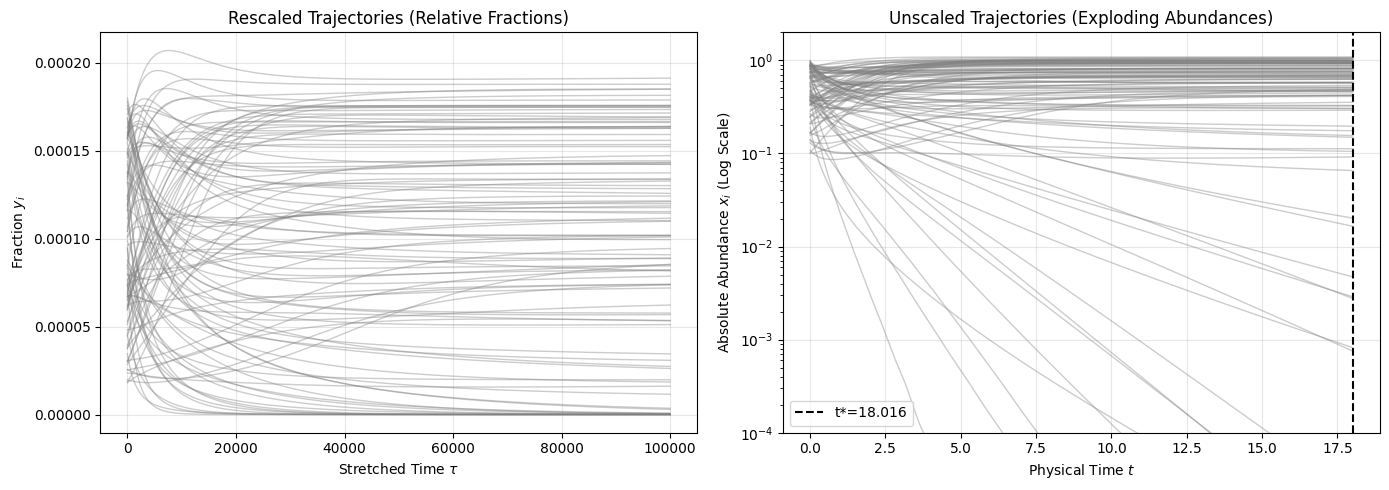
\includegraphics[width=\linewidth]{rescaled_unscaled_mu_minus_2.png}
    \caption{Rescaled (left) and reconstructed unscaled (right) trajectories for
    $N = 10^4$, $C = 50$, $\sigma = 0.5$, and $\mu = -2 < \mu_c \approx 0.5458$.
    The physical abundances relax to a finite stationary state.}
    \label{fig:stable-unscaled}
\end{figure}

\begin{figure}[htbp]
    \centering
    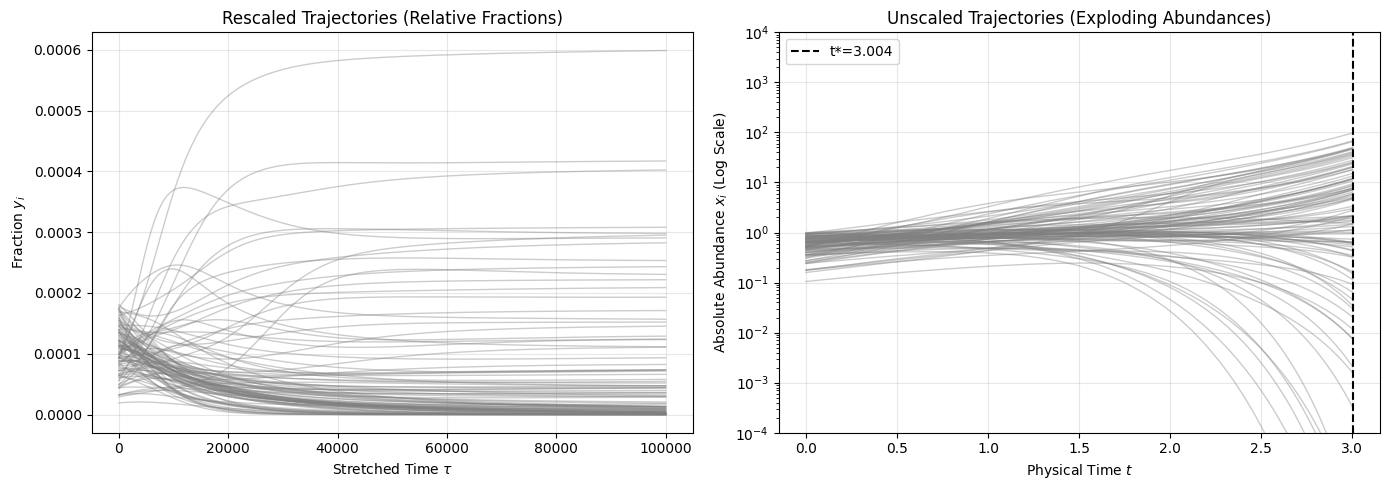
\includegraphics[width=\linewidth]{rescaled_unscaled_mu_05.png}
    \caption{Same parameters as Fig.~\ref{fig:stable-unscaled} but at
    $\mu = 0.5 \approx \mu_c \approx 0.5458$. The simplex dynamics still
    converge, while the reconstructed abundances grow over a much shorter
    physical horizon, signalling the onset of the finite-time divergence of
    $M(t)$.}
    \label{fig:diverging-unscaled}
\end{figure}

\section{Locating the critical point}
\label{sec:locating-muc}

We want the model to behave like an economy: its total size should grow without
bound over time, but it should not explode. This requirement fixes where we operate.
For $\mu < \mu_c$ the total abundance $M$ settles to a finite plateau, so the economy
saturates at a fixed size and stops growing. For $\mu > \mu_c$ the opposite happens:
$M$ diverges in finite physical time, reaching arbitrarily large values at a finite
$t^\ast$, a catastrophic blow-up. The two regimes meet at the critical point $\mu_c$,
where $M$ still grows without bound but its blow-up time is pushed to infinity, so the
growth is unbounded yet as slow as the model allows. We therefore operate at $\mu_c$:
the smallest $\mu$ that gives unbounded growth, and hence the slowest unbounded growth
available. This makes locating $\mu_c$ accurately a prerequisite. We approach it from
two sides: first the mean-field prediction inherited from the literature, and then a
pair of empirical estimators read directly off the rescaled dynamics, which we finally
compare against that prediction.

\section{The theoretical critical point}
\label{sec:theoretical-muc}

The heterogeneous dynamical mean-field theory of Aguirre-L\'opez et al.
\cite{aguirrelopez} yields a closed set of self-consistency equations for the
fixed-point statistics, in which the critical degree $g_c$ controls the
fraction of surviving nodes.

The theory works by reducing the full $N$-node network dynamics to an effective
stochastic process for the abundance $x(t)$ of a single representative node of
rescaled degree $g = k/C$. In the high-connectivity limit this effective process
reads \citep{aguirrelopez}
\begin{equation}
    \dot{x} = x\left( 1 - x + g\mu M(t) + \sqrt{g}\,\sigma\,\eta(t)
              + g\gamma\sigma^2 \int_0^t \mathrm{d}s\, G(t,s)\, x(s) \right),
    \label{eq:dmft-effective}
\end{equation}
where $M(t)$ is the mean abundance, $\eta(t)$ is a Gaussian noise with zero mean
and self-consistent autocorrelation $\langle \eta(t)\eta(s)\rangle =
\langle x(t)x(s)\rangle$, and the retarded friction term encodes the feedback of a
node on itself through the reciprocity $\gamma$ of the couplings. The disorder in
the interactions, once averaged over, thus shows up as a coloured noise whose
statistics must be determined self-consistently from the trajectories it
generates. The kernel of the friction term is the response function
\begin{equation}
    G(t,s) = \left\langle \frac{1}{\sqrt{g}\,\sigma}
             \frac{\delta x(t)}{\delta \eta(s)} \right\rangle,
    \label{eq:response-def}
\end{equation}
the linear response of the abundance at time $t$ to a perturbation of the
effective noise at the earlier time $s$. At a fixed point the statistics become
time-translation invariant, and the two order parameters entering the threshold
equations are the stationary values $q^\ast = \langle x(t)x(t')\rangle$, the
mean-square abundance, and $\chi^\ast = \int_0^\infty G(s)\,\mathrm{d}s$, the
static susceptibility, with $G(s)$ the time-translation-invariant limit of
$G(t,\,t-s)$.

The threshold $\mu_c$ is the value of $\mu$ at
which $g_c \to 0$, i.e.\ at which even the least-connected nodes are about to be
driven extinct in the relative variables. Setting $g_c = 0$ in the
self-consistency relations gives
\begin{equation}
\begin{aligned}
1 &= |\mu| \int_0^{g^*} \mathrm{d}g\, \nu(g)\, g\, \frac{\sqrt{g q^*}\, \sigma}{1 - g\gamma\sigma^2\chi^*} \int_{-\Delta_g}^{\infty} Dz\, (\Delta_g + z), \\
1 &= \int_0^{g^*} \mathrm{d}g\, \nu(g)\, g\, \frac{g\sigma^2}{(1 - g\gamma\sigma^2\chi^*)^2} \int_{-\Delta_g}^{\infty} Dz\, (\Delta_g + z)^2, \\
\chi^* &= \int_0^{g^*} \mathrm{d}g\, \nu(g)\, g\, \frac{1}{1 - g\gamma\sigma^2\chi^*} \int_{-\Delta_g}^{\infty} Dz, \\
\Delta_g &= \operatorname{sgn}(\mu)\, \frac{g - g_c}{\sqrt{g q^*}\, \sigma}, \qquad
g^* = \frac{1}{|\gamma|\, \sigma^2 \chi^*\, \theta(\gamma)},
\end{aligned}
\label{eq:muc-selfconsistency}
\end{equation}
with $Dz = e^{-z^2/2}\,dz/\sqrt{2\pi}$ the standard Gaussian measure, and
$q^\ast$, $\chi^\ast$ the fixed-point order parameters introduced above. The
remaining symbols are structural: $\gamma = \overline{z_{ij} z_{ji}}$ is the
reciprocity of the couplings (interpolating from fully antisymmetric,
$\gamma = -1$, through uncorrelated, $\gamma = 0$, to symmetric, $\gamma = +1$);
$\nu(g)$ is the rescaled degree distribution, $\nu(g) = \lim_{C\to\infty}
\sum_k p(k)\, \delta(g - k/C)$, with $g = k/C$ the degree in units of the mean
connectivity; and $\theta(\cdot)$ is the Heaviside step. In the
noiseless limit these collapse to the familiar $\mu_c = 1/\langle g^2 \rangle$;
for $\sigma > 0$ the disorder shifts the threshold, and solving
\eqref{eq:muc-selfconsistency} numerically traces out $\mu_c(\sigma)$ for the
exponential degree distribution.

The role of the degree distribution itself can be isolated here. The
threshold depends on $\nu(g)$ only through its moments, in the noiseless limit
through $\langle g^2 \rangle$ alone, so the natural reference is a regular
graph, with every node at the mean degree, $\nu(g) = \delta(g - 1)$, carrying the
same mean $\langle g \rangle = 1$ as the exponential ensemble but zero degree
variance. Contrasting the two isolates the effect of heterogeneity itself. For a
single degree the outer integral in \eqref{eq:muc-selfconsistency} collapses to
its integrand at $g = 1$, and the self-consistency system reduces to a
one-dimensional root condition. Figure~\ref{fig:mu_comparison} traces
$\mu_c(\sigma)$ for both. At $\sigma = 0$ the regular
graph sits at $\mu_c = 1/\langle g^2 \rangle = 1$, exactly twice the exponential
value of $1/2$, and it stays above the exponential curve at every $\sigma$, with
the gap widening as the disorder grows. The reading is that degree heterogeneity
lowers the cooperative threshold: a broad spread of connectivities lets
the best-connected nodes drive the macroscopic abundance to divergence at a
weaker mean interaction than a uniform network would require, making the
heterogeneous system the more fragile of the two.

\begin{figure}[h]
    \centering
    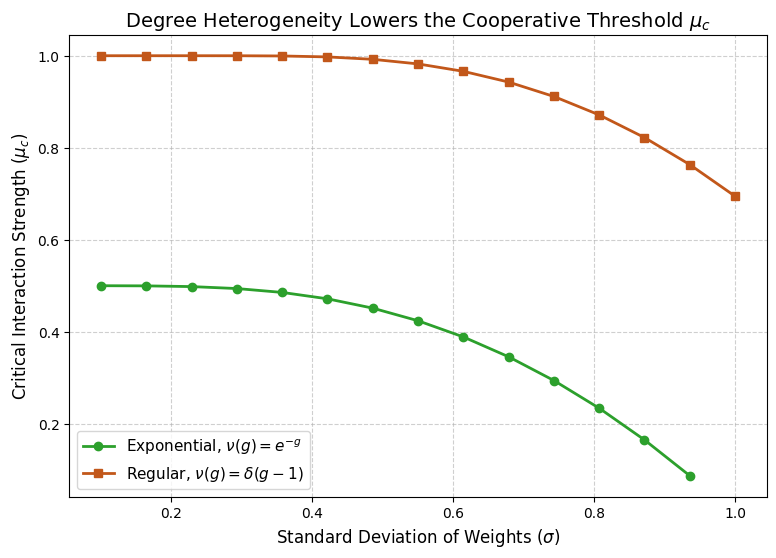
\includegraphics[width=0.75\linewidth]{mu_c_scaling_comparison.png}
    \caption{Numerical solution of \eqref{eq:muc-selfconsistency} for the
    critical interaction strength $\mu_c$ as a function of the disorder strength
    $\sigma$, for an exponential degree distribution $\nu(g) = e^{-g}$ (green
    circles) and a regular graph $\nu(g) = \delta(g - 1)$ (orange squares), both
    at $\gamma = 0$ and shared mean degree $\langle g \rangle = 1$. With no
    degree variance the regular graph lies above the heterogeneous one
    throughout, starting from the noiseless value $\mu_c = 1$; the separation
    grows with $\sigma$.}
    \label{fig:mu_comparison}
\end{figure}

\section{Empirical estimators of $\mu_c$ on finite graphs}
\label{sec:empirical-muc}

The mean-field prediction \eqref{eq:muc-selfconsistency} assumes the
thermodynamic limit and the associated degree statistics. On a finite graph the
true threshold is shifted, and since we need to sit at $\mu_c$ this shift
matters. We therefore measure $\mu_c$ directly from the rescaled dynamics, by sweeping $\mu$
across the threshold and averaging, at each value, over several realizations of the
random graph, its couplings, and the initial condition. A single integration yields
two observables at once, the asymptotic shape scalar $c$ and the saturating physical
time $t_{\mathrm{final}}$, so the sweep delivers two estimators of $\mu_c$ rather than
one. The first reads the sign of the divergence directly off the
relaxed shape; the second detects the same transition through its integrated
effect on physical time. We describe each in turn and then compare them.

\subsection{The shape scalar $c$}
\label{sec:estimator-c}

The cleanest estimator needs only the shape dynamics. We integrate the shape
equation \eqref{eq:dydtau} on its own, which is closed in $y$ and stays bounded,
until it relaxes to its fixed point $y^\ast$, and read off the scalar
\begin{equation}
    c \equiv (y^\ast)^{\!\top} W y^\ast - (y^\ast)^{\!\top} y^\ast .
    \label{eq:c-scalar}
\end{equation}
The sign of $c$ marks the threshold: as derived in
Section~\ref{sec:simplex-mapping}, $c < 0$ below the critical point and $c > 0$
above it, so $\mu_c$ is the zero crossing of $c(\mu)$. We locate it with a
one-dimensional root find, a Brent bracket on a coarse $\mu$-grid refined per
realization. Because $c$ is a property of the relaxed shape alone, it is fixed as
soon as $y(\tau)$ reaches its plateau, which a modest $\tau_{\max}$ reaches; the
shape integration stays bounded and cannot overflow, so the estimator is cheap and
numerically benign, and no scale equation needs to be integrated for it.

The estimator rests on one premise: that the shape actually relaxes to a fixed
point, so that $c$ is a well-defined late-time constant. This holds only in the
single-fixed-point phase; for strong enough disorder the shape never settles and
the sign-of-$c$ reading is ill-posed. Figure~\ref{fig:shape-relaxation} maps the
boundary directly, recording per cell the fraction of realizations whose shape
velocity $\lVert\dot y\rVert$ falls to the solver floor (relaxation) over the
$(\mu,\sigma)$ plane, for both topologies and a range of mean degree $C$. The
relaxed (green) region covers the entire operating box used in
Chapter~\ref{chap:results} ($\sigma = 0.2$, $\mu$ at the per-topology
$\mu_c^{\mathrm{th}}$) with wide margin; non-relaxation is confined to a strip at
$\sigma \gtrsim 1$ that the exponential graph enters slightly earlier than the
regular one, its hubs destabilizing first. The estimator is therefore used
strictly inside its domain of validity, and relaxation is in practice confirmed
post hoc (vanishing $\lVert\dot y\rVert$ at $\tau_{\max}$) in every reported run.

\begin{figure}[htbp]
    \centering
    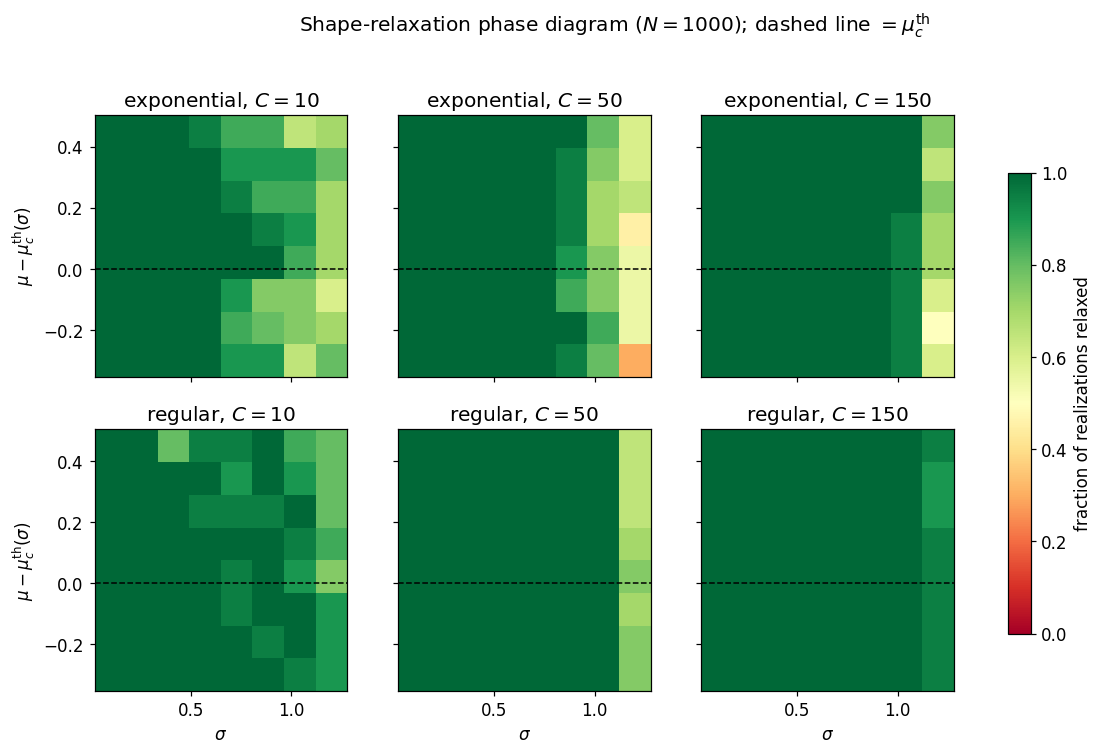
\includegraphics[width=\linewidth]{shape_relaxation_phase.png}
    \caption{Shape-relaxation phase diagram at $N = 1000$. Each cell gives the
    fraction of realizations whose shape velocity decays to the solver floor,
    over the $(\mu,\sigma)$ plane (with $\mu$ measured relative to the
    per-topology $\mu_c^{\mathrm{th}}$, dashed line), for the exponential (top) and
    regular (bottom) graphs at mean degree $C \in \{10, 50, 150\}$. The shape
    relaxes (green, $c$ well-defined) across the whole operating region; the
    non-relaxing strip (red/yellow) sits at $\sigma \gtrsim 1$, well above the
    $\sigma = 0.2$ used in the results.}
    \label{fig:shape-relaxation}
\end{figure}

\subsection{The final-time drop}
\label{sec:estimator-tfinal}

The second estimator trades cost for robustness. The procedure follows
immediately from the asymptotics of $M(\tau)$ derived in
Section~\ref{sec:simplex-mapping}, Eq.~\eqref{eq:M-asymptotics}: we integrate
the rescaled system up to a fixed, large rescaled horizon $\tau_{\max}$ for a
range of $\mu$, and record the corresponding physical time
$t_{\mathrm{final}} = t(\tau_{\max})$. Below the threshold $M$ plateaus, so
$dt/d\tau = 1/M$ stays finite and $t_{\mathrm{final}}$ grows essentially
linearly with $\tau_{\max}$; above it $M \sim e^{c\tau}$, so $1/M$ decays
exponentially and $t(\tau)$ saturates at the finite blow-up time $t^\ast$. The
two regimes are distinguished by their dependence on the horizon: below
threshold $t_{\mathrm{final}}$ scales with $\tau_{\max}$, above it sits on a
$\tau_{\max}$-independent floor. The empirical $\mu_c$ is therefore read off as
the onset of that flat floor, the point at which $t_{\mathrm{final}}$ stops
scaling with the horizon, which is exactly the $c = 0$ condition. It is not read
as the midpoint of the visible drop, which the inflated subcritical branch
biases low (Fig.~\ref{fig:empirical-muc}).

\begin{figure}[h]
    \centering
    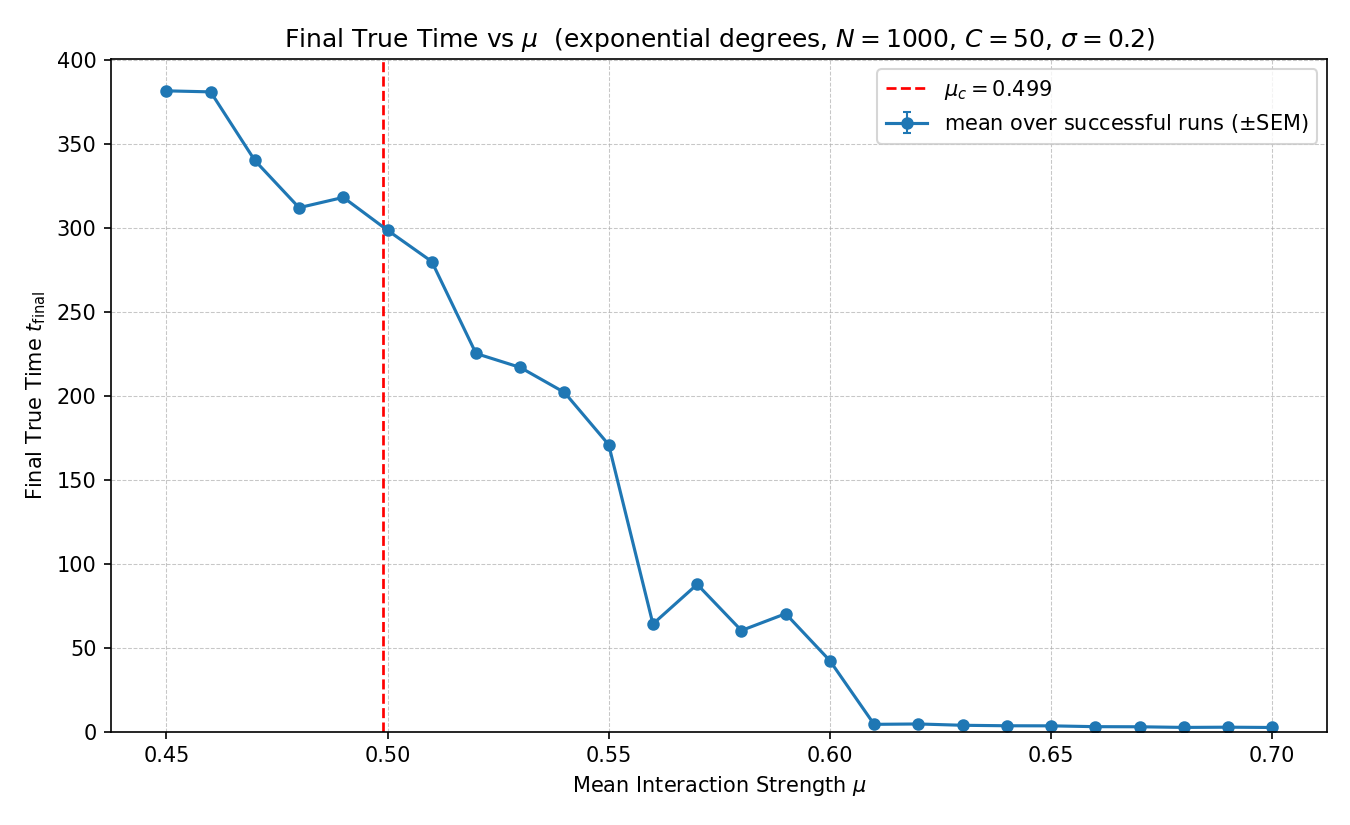
\includegraphics[width=\linewidth]{true_mu_c.png}
    \caption{Final physical time $t_{\mathrm{final}} = t(\tau_{\max})$ versus
    mean interaction strength $\mu$, with $\tau_{\max} = 10^6$. In the
    subcritical regime $M$ plateaus at $-1/c$, so
    $t_{\mathrm{final}} \approx (-c)\,\tau_{\max}$ grows with the horizon and
    its slope flattens as $\mu$ rises and $c \to 0^-$; this descending ramp is
    a horizon-inflated quantity, not a fixed level. Above the critical point
    $M$ diverges exponentially and $t_{\mathrm{final}}$ saturates at the finite
    blow-up time $t^\ast$, independent of $\tau_{\max}$. The empirical $\mu_c$
    is therefore read as the onset of this flat, horizon-independent floor,
    near $\mu \approx 0.61$, not the midpoint of the visible drop, which is
    biased low by the $\tau_{\max}$-inflated subcritical ramp. Points are means
    over successful runs ($\pm$ SEM); parameters $N = 1000$, $C = 50$,
    $\sigma = 0.2$, exponential degree distribution. The dashed line marks the
    mean-field prediction $\mu_c = 0.499$.}
    \label{fig:empirical-muc}
\end{figure}

The estimator is robust by construction. Because $t_{\mathrm{final}}$ is the
integral of $1/M(\tau)$, it accumulates the entire history of the
trajectory rather than relying on a single late-time value, so even a slowly
diverging $M(\tau)$, the hardest case to detect and the regime of greatest
interest, is registered cleanly. The observable also comes at no extra cost: it is a
byproduct of the same integration that produces $y(\tau)$, requiring no
additional computation.


\subsection{Comparing the two estimators}
\label{sec:estimator-comparison}

Comparing the two estimators is not a trade-off: the shape scalar $c$ is the sounder
and faster of the two. It reads the critical condition directly off the relaxed
shape, needs only a modest $\tau_{\max}$, and costs a few hundred solver steps. The
final-time drop reaches the same condition indirectly, by integrating $1/M(\tau)$
until $M$ has genuinely diverged, so it needs a much larger $\tau_{\max}$ and is
located less cleanly. We run it only as an independent check on $c$: we locate
$\mu_c$ with both across many realizations and a range of horizons $\tau_{\max}$,
asking of each the same three questions: is it flat in $\tau_{\max}$ (insensitive to
the cutoff), is its realization-to-realization spread small, and does it sit on the
mean-field reference? Once they converge to the same value, we use $c$. Capping the abundance $M$ at a fixed value, well below the floating-point ceiling,
is what makes this sweep possible at all: it keeps the supercritical runs finite and
fills in the part of the $\mu$-range where an uncapped solver would return only
\texttt{NaN}s.

Figure~\ref{fig:estimator-comparison} and Table~\ref{tab:estimator-comparison}
report this sweep. The shape scalar $c$ converges almost immediately: it has
settled by $\tau_{\max} \approx 10^4$ to $\mu_c \approx 0.617$ and is flat for
every larger horizon, with a stable spread of about $0.023$ and at a cost of only
a few hundred solver steps. The final-time drop is slower and more erratic. It
overshoots badly at the shortest horizon ($0.85$ at $\tau_{\max} = 10^3$), then
settles only around $\tau_{\max} \approx 5\times10^5$ onto its own plateau at
$\mu_c \approx 0.585$, an order of magnitude more steps later. The two
estimators are in fact reading the same condition (the sign change of $c$) in two
different ways, and the residual gap between them ($0.617$ for $c$
against $0.585$ for the drop) is not intrinsic but an artifact of how the drop
is located. The steepest-descent point interpolates between the supercritical
floor and a subcritical level that, because $t_{\mathrm{final}} \approx
(-c)\,\tau_{\max}$ in that regime, is inflated by the horizon, so the midpoint
is pulled below the true $c = 0$ crossing. This is also why the drop drifts
upward with $\tau_{\max}$ (from $0.510$ at $\tau_{\max} = 10^4$ to $0.585$): as
the horizon grows the inflated branch steepens and the steepest-descent point
shifts toward the crossing. It stalls at $0.585$, short of the $c$ value,
because the tanh midpoint remains a biased functional of the inflated curve no
matter how far $\tau_{\max}$ is pushed. Locating $t_{\mathrm{final}}$ instead by
the onset of its flat, $\tau_{\max}$-independent floor closes that residual gap by
construction. That onset is the operational form of ``$t_{\mathrm{final}}$ has
stopped scaling with the horizon,'' which is exactly $c = 0$, so the floor onset
is the $c = 0$ crossing itself. The shape scalar $c$ simply reaches the same
conclusion directly, off the relaxed shape, without the detour through
$t_{\mathrm{final}}$. Both estimators lie above the mean-field
value $\mu_c = 0.5$, a positive finite-size bias examined in the next section.
Because the $c$ zero-crossing
is both the more principled estimator and by far the cheaper and more stable one,
we adopt it as our working estimator in what follows.

\begin{figure}[h]
    \centering
    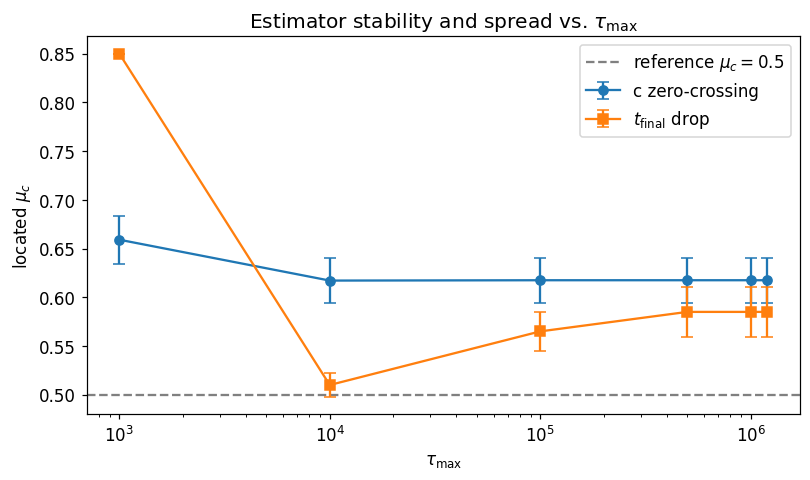
\includegraphics[width=0.85\linewidth]{estimator-convergence-comparison.png}
    \caption{Located critical point $\mu_c$ from the two estimators (the shape
    scalar $c$ zero-crossing and the $t_{\mathrm{final}}$ drop) as a function of
    the rescaled horizon $\tau_{\max}$, averaged over realizations ($\pm$ spread).
    The $c$ estimator converges by $\tau_{\max} \approx 10^4$ and is flat
    thereafter; the $t_{\mathrm{final}}$ drop drifts upward with the horizon and
    plateaus at $\mu_c \approx 0.585$, short of the $c$ value because the
    drop-midpoint locator stays biased by the horizon-inflated subcritical
    branch. Both lie above the mean-field
    reference $\mu_c = 0.5$ (dashed) by the finite-size bias. Parameters
    $N = 1000$, $C = 50$, $\sigma = 0.2$, exponential degree distribution.}
    \label{fig:estimator-comparison}
\end{figure}

\begin{table}[h]
    \centering
    \begin{tabular}{rccr}
        \hline
        $\tau_{\max}$ & $c$ zero-crossing & $t_{\mathrm{final}}$ drop & mean steps \\
        \hline
        $10^3$         & $0.659 \pm 0.025$ & $0.850 \pm 0.000$ &    384 \\
        $10^4$         & $0.617 \pm 0.023$ & $0.510 \pm 0.012$ &    741 \\
        $10^5$         & $0.618 \pm 0.023$ & $0.565 \pm 0.020$ &   7589 \\
        $5\times10^5$  & $0.618 \pm 0.023$ & $0.585 \pm 0.026$ &  31357 \\
        $10^6$         & $0.618 \pm 0.023$ & $0.585 \pm 0.026$ &  64267 \\
        $2\times10^6$  & $0.618 \pm 0.023$ & $0.585 \pm 0.026$ &  94316 \\
        \hline
    \end{tabular}
    \caption{Located $\mu_c$ from the two estimators as a function of the rescaled
    horizon $\tau_{\max}$ (mean $\pm$ standard deviation over realizations),
    together with the mean number of solver steps per $\mu$-sweep. The $c$
    zero-crossing is converged and stable from $\tau_{\max} = 10^4$ at a few
    hundred steps, while the $t_{\mathrm{final}}$ drop settles only near
    $\tau_{\max} = 5\times10^5$ and at roughly two orders of magnitude more steps.
    Parameters as in Fig.~\ref{fig:estimator-comparison}.}
    \label{tab:estimator-comparison}
\end{table}

\FloatBarrier

\section{Comparison with the theoretical prediction}
\label{sec:muc-statistics}

Having adopted the shape scalar $c$ (Section~\ref{sec:estimator-comparison}), we now
compare the empirical threshold it gives against the mean-field prediction of
Section~\ref{sec:theoretical-muc}. The empirical threshold fluctuates from one graph
realization to the next, and it is biased relative to the mean-field value.
Figure~\ref{fig:distribution_muc} shows the distribution of the gap
$\mu_c^{\mathrm{emp}} - \mu_c^{\mathrm{th}}$ over $100$ independent realizations,
located with $c$: at this operating point ($N = 1000$, $C = 50$, $\sigma = 0.2$) the
mass concentrates at positive values, with a mean of $0.0974$, so the empirical
estimator overestimates $\mu_c$ on average. The sign of this gap is not universal,
however: as Figure~\ref{fig:finite_size} shows, it depends on the mean degree $C$,
the system size $N$, and the disorder $\sigma$, and the empirical threshold can lie
either above or below the mean-field value.

\begin{figure}[h]
    \centering
    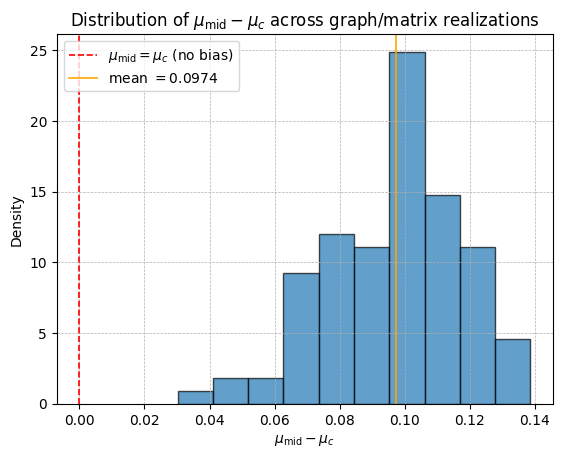
\includegraphics[width=0.75\linewidth]{theoretical-vs-actual.png}
    \caption{Distribution of the distance between the measured and predicted
    critical points, $\mu_c^{\mathrm{emp}} - \mu_c^{\mathrm{th}}$, over $100$
    realizations with $N = 1000$, $C = 50$, $\sigma = 0.2$ on an exponential
    graph. The positive mean ($0.0974$) shows a systematic overestimation of
    $\mu_c$ at this operating point.}
    \label{fig:distribution_muc}
\end{figure}

The size of this bias is controlled by how closely the finite graph satisfies
the assumptions behind \eqref{eq:muc-selfconsistency}, which is derived in the
double limit $1 \ll C \ll N$: each node must see enough neighbours for its local
field to be Gaussian, while the graph stays sparse enough to remain locally
tree-like. At fixed $N$ these two demands compete as $C$ grows. Sweeping $C$ with
all other parameters fixed shows the gap for the exponential graph rising with
$C$: it is slightly negative at small $C$, crosses zero, and is clearly positive by
$C = 150$ ($N = 1000$, $\sigma = 0.2$), as the exponential panels of
Fig.~\ref{fig:finite_size} make plain. The reason is that at $N = 1000$ a connectivity of $C = 150$ is no
longer small compared with the system: the ratio $C/N$ approaches unity, the
sparse tree-like structure the theory assumes is lost, and the prediction
degrades. Increasing $C$ at fixed $N$ therefore moves away from the regime
where the mean field is exact, not toward it; the genuine limit is approached by
growing $N$, as we show next.

That the relevant limit is in $N$ rather than $C$ is confirmed by resolving the
gap across system size. Figure~\ref{fig:finite_size} sweeps $C$ at three sizes
$N \in \{1000, 2000, 5000\}$ and three disorder strengths, for both the
exponential graph and a regular graph in which every node carries the mean
degree. To keep this broad sweep affordable we use the shape-scalar estimator
throughout, which is far cheaper than the drop. For the exponential graph the gap grows with $C$ at every
$N$, but at fixed $C$ it shrinks with $N$, roughly halving with each
doubling of $N$, so the curves decrease toward zero: the mean-field value is
recovered by enlarging the system at fixed connectivity, which restores
$C \ll N$. The effect is essentially independent of $\sigma$, marking the
correction as structural. The regular graph behaves the other way, and with the
opposite sign: the gap is identically zero at $\sigma = 0$, and at $\sigma = 0.2$ and
$\sigma = 0.4$ it is negative, largest at small $C$ and high disorder and closing
toward zero as $C$ grows. On a homogeneous graph the empirical threshold therefore
sits slightly below the mean-field value, not above it. The large, $N$-sensitive
correction that grows with $C$ is thus specific to degree heterogeneity, while the
homogeneous graph carries only a small negative residual.

\begin{figure}[h]
    \centering
    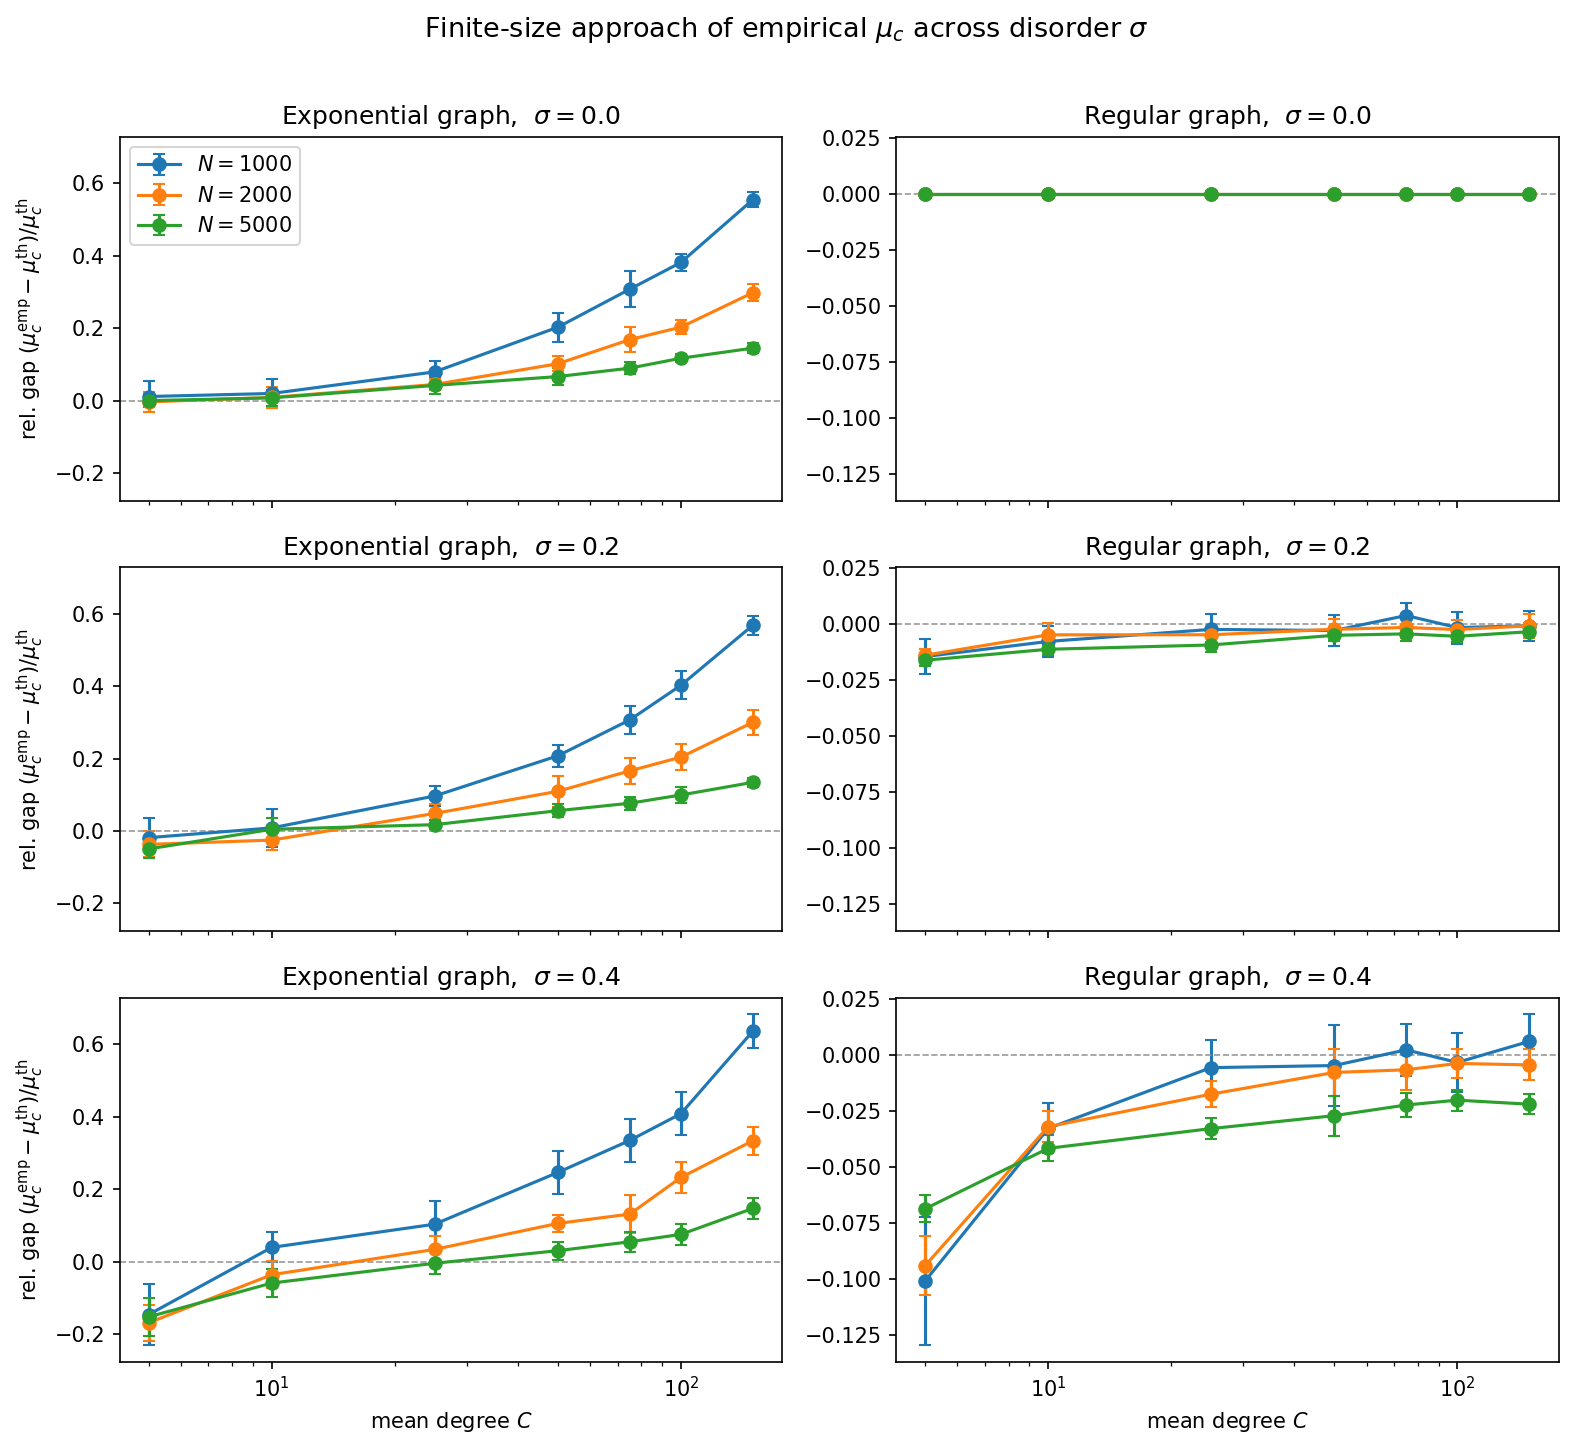
\includegraphics[width=\linewidth]{mu_c_finite_size.png}
    \caption{Relative gap
    $(\mu_c^{\mathrm{emp}} - \mu_c^{\mathrm{th}})/\mu_c^{\mathrm{th}}$ versus mean
    degree $C$ for the exponential (left) and regular (right) graphs, at disorder
    strengths $\sigma = 0, 0.2, 0.4$ (rows) and sizes $N = 1000, 2000, 5000$
    (colours); shape-scalar estimator, mean $\pm$ std over realizations. Note the
    differing vertical scales between the two columns. The exponential gap grows
    with $C$ and shrinks with $N$, converging to the mean field as $N \to
    \infty$; the regular gap stays near zero throughout and vanishes identically
    at $\sigma = 0$. Degree heterogeneity is the dominant source of the
    finite-size correction.}
    \label{fig:finite_size}
\end{figure}